\newcommand{\CLASSINPUToutersidemargin}{0.5in}
\documentclass[a4paper,conference]{IEEEtran}
\IEEEoverridecommandlockouts
% The preceding line is only needed to identify funding in the first footnote. If that is unneeded, please comment it out.
\usepackage{cite}
\usepackage{amsmath,amssymb,amsfonts}
\usepackage{algorithmic}
\usepackage{graphicx}
\usepackage{textcomp}
\usepackage{xcolor}
\usepackage{xurl}
\usepackage{hyperref}
\hypersetup{
    colorlinks = true,
    linkcolor = [rgb]{.1,.1,.44},
    urlcolor = blue,
    citecolor = [rgb]{.0,.39,.0}
}
\usepackage{listings}
\usepackage{color}
\definecolor{dkgreen}{rgb}{0,0.6,0}
\definecolor{gray}{rgb}{0.5,0.5,0.5}
\definecolor{mauve}{rgb}{0.58,0,0.82}
\lstset{frame=tb,
  language=Java,
  aboveskip=3mm,
  belowskip=3mm,
  showstringspaces=false,
  columns=flexible,
  basicstyle={\small\ttfamily},
  numbers=none,
  numberstyle=\tiny\color{gray},
  keywordstyle=\color{blue},
  commentstyle=\color{dkgreen},
  stringstyle=\color{mauve},
  breaklines=true,
  breakatwhitespace=true,
  tabsize=3
}
\def\BibTeX{{\rm B\kern-.05em{\sc i\kern-.025em b}\kern-.08em
    T\kern-.1667em\lower.7ex\hbox{E}\kern-.125emX}}
\begin{document}

\renewcommand\footnoterule{{\hrule height 0.5pt}\vspace{0.04in}}
\def\IEEEkeywordsname{Keywords}

\title{Huffman Coding Homework\\
\vspace{-0.1in}
{\normalsize Authors Name, Student ID}
}

\author{}

\maketitle

% \begin{abstract}
% \end{abstract}

\vspace{0.1in}

\begin{IEEEkeywords}
Huffman Algorithm; Adaptive Huffman Algorithm; FGK Algorithm; Data Compression
\end{IEEEkeywords}

\section{Introduction}
In this homework, I implement the basic Huffman algorithm, adaptive Huffman algorithm and some limited extended Huffman algorithm in C++, and compare the performance of them. The basic Huffman algorithm only work when entire files is given to compute the probability mass function of each symbol. The adaptive Huffman algorithm can work when the file is streaming, which means the probability of each symbol is not given. The entropy of file is the minimum number of bits needed to represent symbol. The best compression ratio using basic Huffman algorithm is is $72.1\%$, which threat file as $32$-bit source.

\section{Basic Huffman Algorithm}

In basic Huffman algorithm, the probability mass function of each symbol is given, and the Huffman tree is built by the probability mass function. The Huffman code can be proven to be optimal, which means the average codeword length is minimum. The Huffman code is a prefix code, variable length code and instanous code.

\subsection{Huffman Tree}

The Huffman tree is binary tree, the leaf node contain the symbol and its probability, the internal node contains the sum of its children's probability.

I have implemented a Huffman tree using C++ template, $HuffmanTree<logD, V>$, which allows for some flexibility in modifying the tree to a d-ary Huffman tree or changing value type to big-integer to implement the extended Huffman algorithm.

To construct the Huffman tree from the probability of symbols, I use heap data structure $std::priority\_queue$ and array index instead of pointer to construct the tree more efficiency.

To encode the file, I utilize a hash table, using $std::unordered\_map$, to map symbols to their respective codewords.

To decode the file, I treat the file as a bit stream, and traverse the Huffman tree bit by bit, until find the symbol corresponding to given bits sequence.

\subsection{Huffman Tree Storage}

When compressing and decompressing a file using the basic Huffman algorithm, the Huffman tree is required to encode and decode the file. The Huffman tree can be stored in the file header, or in a separate file. I have choosen to store it in the file header using the method described in \cite{efficient-way-of-storing-Huffman-tree}. The method involves a pre-order traversal of the tree, where an internal node is stored as $0$, followed by a recursive storage of its child nodes, and a leaf node is stored as $1$, and followed by the symbol that it represents.

\subsection{Compressed File Format}

The compressed file format is a binary file that includes both the Huffman tree and the encoded file. It starts with a $32$-bit integer, denoted as $k$, which represents the number of bits in the Huffman tree. Following this, the Huffman tree itself is stored in the next $k$ bits. After the Huffman tree, a $32$-bit integer $n$ is included, which represents the number of bytes in the original file. Finally, the encoded file is stored after $n$.

\section{Adaptive Huffman Algorithm}

The adaptive Huffman algorithm is a variance of the basic Huffman algorithm, which can work when the file is streaming. The adaptive Huffman tree is built by the occurrence of already transmitted symbols, and update the code tree when every symbol is transmitted. There are two notable implementation of adaptive Huffman algorithm, the FGK algorithm and the Vitter algorithm. The FGK algorithm is a simple algorithm, and mentioned in Textbook \cite{Introduction to Data Compression}. The Vitter algorithm is a more efficient algorithm, and mentioned in Wiki \cite{Wiki Adaptive_Huffman_coding}. I have implemented the FGK algorithm in this homework.

\subsection{FGK Algorithm}

The FGK algorithm would update code tree when every symbol is transmitted. The code tree is built by the occurrence of already transmitted symbols. The code tree is a binary tree, the leaf node contain the symbol and its occurrence, the internal node contains the sum of its children's occurrence. There are two special nodes, the root node and the NYT (not yet transmitted) node. The root node is the root of the code tree, and the NYT node indicate the symbol that has not been transmitted yet, then transmitted symbol via $[ \log_2{|\Omega|} ]$-bits fixed length code.

I have implemented a FGK Algorithm using C++ template, $HuffmanTreeFGK<logD, V, NYTvalue>$, which allows for some flexibility in modifying the tree to a d-ary Huffman tree or changing value type to big-integer to implement the extended Huffman algorithm, and reserve the NYT value to be any value in V type, and use array index instead of pointer to construct the tree want more efficiency.

To encode the file, I utilize a hash table, using $std::unordered\_map$, to map symbols to their respective index in the code tree.

To decode the file, I treat the file as a bit stream, and traverse the Huffman tree bit by bit, until find the symbol corresponding to given bits sequence or the NYT node.

\subsection{FGK Algorithm -- Update}

When the new symbol is transmitted, the NYT node will become internal node, and its child would new NYT node and new symbol node, then follow the update procedure same as the existing symbol.
When the existing symbol is transmitted, the node would swap with the node which has highest order and same occurrence, then repeat the procedure until the node is the root node.

\subsection{FGK Algorithm -- Encode}

When the new symbol is transmitted, send the code for NYT node, then send the fixed length code of the new symbol. When the existing symbol is transmitted, send the code for the node of the symbol. Then follow the update procedure to update the code tree.

\subsection{FGK Algorithm -- Decode}

When the code is decoded to NYT node, then the next $[ \log_2{|\Omega|} ]$-bits code is the new symbol. When the code is decoded to existing node, then the symbol on its leaf node. Then follow the update procedure to update the code tree.

\section{Extended Huffman Algorithm}

The extended Huffman algorithm is group $n$ symbols into extended symbol, in theory, this method would make average codeword length closed to entropy when symbols is independent and identically distributed.

In this homework, I have implemented the limited version of extended Huffman algorithm with $8 \le n = 8k \le 64$, and $k$ is a positive integer.


\begin{figure}[htbp]
\centerline{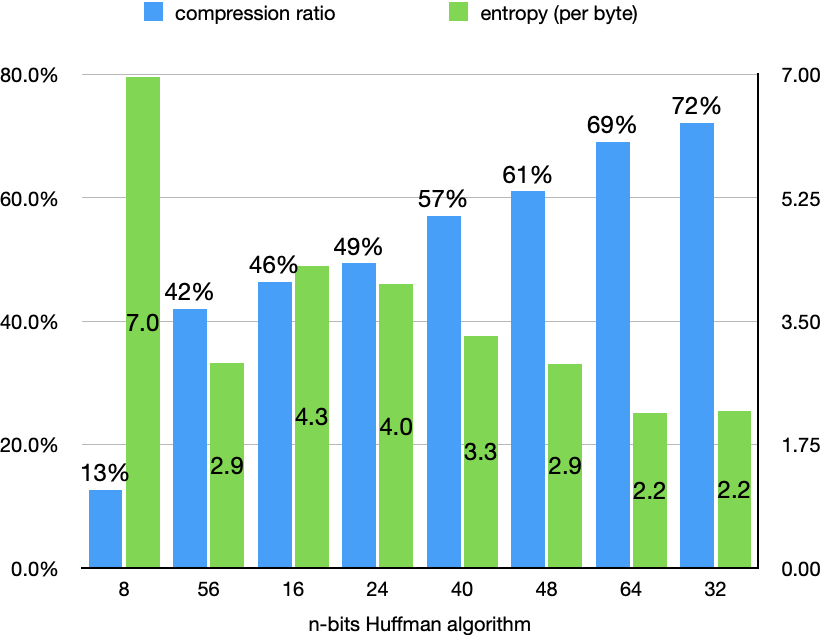
\includegraphics[height=6.15cm, keepaspectratio,]{assets/chart-entropy-compression-ratio-asc.png}}
\caption{The entropy and compression ratio of $n$-bits Huffman code.}
\label{fig-chart-entropy-compression-ratio}
\end{figure}

\section{Experimental Results}

\subsection{Basic Huffman Algorithm}

The entropy and compression ratio using basic Huffman algorithm, treat file as different bits data source shown in Fig.~\ref{fig-chart-entropy-compression-ratio}.

We can see that for $n$-bits Huffman algorithm, the entropy of file per byte ($\frac{H(X)}{n}$) is inverse proportional to the compression ratio, except for $56$-bits Huffman algorithm.

When we only consider the file without header, the entropy of file per byte is more close to inverse proportional to the compression ratio, shown in Fig.~\ref{fig-chart-entropy-compression-ratio-exclude}, a little exception for $56$-bits.

\begin{figure}[htbp]
\centerline{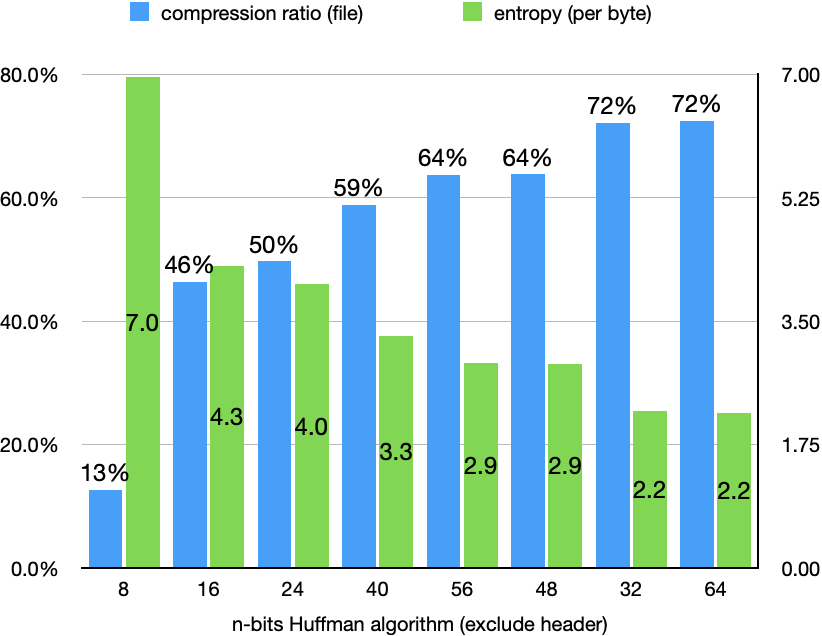
\includegraphics[height=6.15cm, keepaspectratio,]{assets/chart-entropy-compression-ratio-asc-exclude.png}}
\caption{The entropy and compression ratio of $n$-bits Huffman code w/o header.}
\label{fig-chart-entropy-compression-ratio-exclude}
\end{figure}

\subsection{Extended Huffman Algorithm}

Threat source file as $n$-bits stream is limited version of extended Huffman algorithm, because some technique issue in my implementation, the program only support $n$ is mutiple of $8$ from $8$ to $64$. We can view the source as $8$-bits stream, and $n$-bits are extended Huffman code.

\begin{figure}[htbp]
\centerline{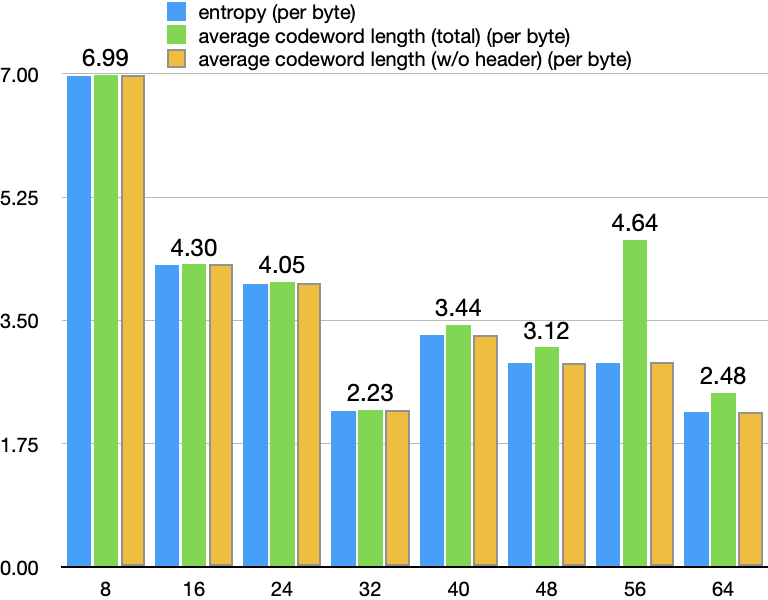
\includegraphics[height=6.15cm, keepaspectratio,]{assets/chart-entropy-average-codeword-length-per-byte.png}}
\caption{The entropy and average codeword length per byte.}
\label{fig-chart-entropy-average-codeword-length-per-byte}
\end{figure}

As the result shown in Fig.~\ref{fig-chart-entropy-compression-ratio}, Fig.~\ref{fig-chart-entropy-compression-ratio-exclude} and Fig.~\ref{fig-chart-entropy-average-codeword-length-per-byte}, we can see that the entropy of file per byte very close to the average codeword length per byte (without header), and as the $n$ increase, the average codeword length per byte (include header) is more higher than the entropy of file per byte.

See Fig.~\ref{fig-chart-alphabet-size-tree-size-height}, $32$-bits makes the smallest alphabet size, so its get highest compression ratio. We can also conclude that the alphabet size is proportional to the tree size, and doesn't affect the height of the tree.

\begin{figure}[htbp]
\centerline{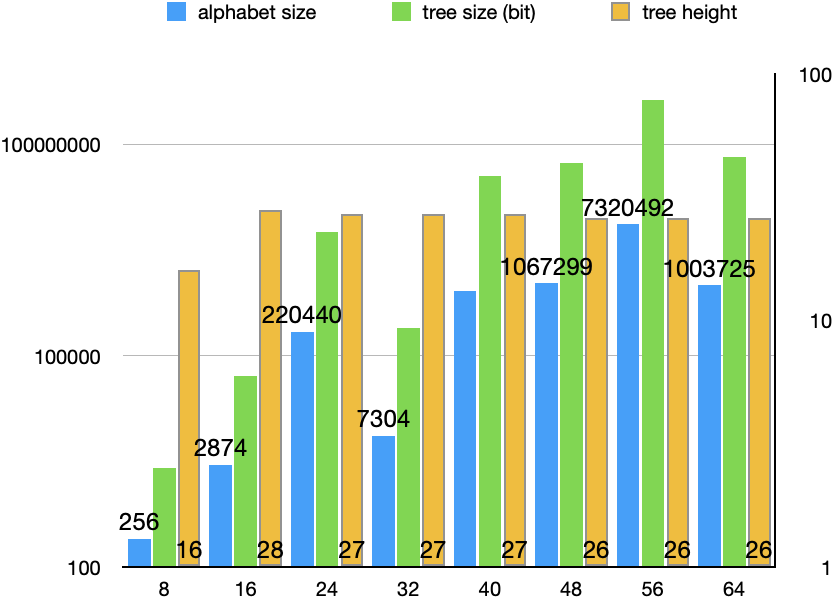
\includegraphics[height=6.15cm, keepaspectratio,]{assets/chart-alphabet-size-tree-size-height.png}}
\caption{The charset}
\label{fig-chart-alphabet-size-tree-size-height}
\end{figure}


\subsection{Basic Huffman Algorithm -- Split every 40MB}

The p.m.f maybe change when the file size is large, so we can split the file into several parts, and encode echo part separately.

Due to some implementation issue, there are some padding in the compressed file, the program I have implemented only allow to split the filesize $fsz$ and treat $n$-bits source stream, where $fsz$ is mutiple of $n$ and $n$ is mutiple of $8$ from $8$ to $64$.

As the result shown in Fig.~\ref{fig-chart-compression-ratio-split}, we can see that the compression ratio between entire file and split every 40MB is very close, only $40$-bits and $64$-bits have a little difference, so we can conclude that the p.m.f doesn't change through $alexnet.pth$ when $n$ less or equal to $32$.

\begin{figure}[htbp]
\centerline{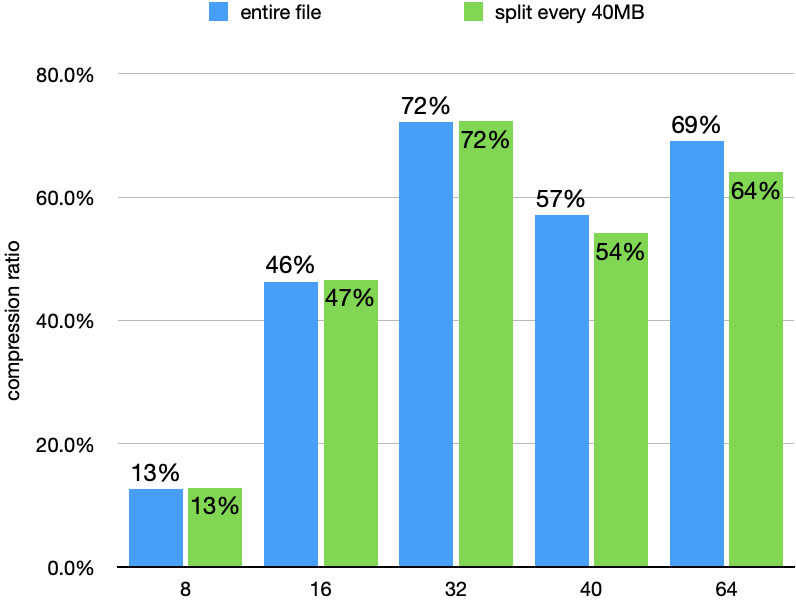
\includegraphics[height=6.15cm, keepaspectratio,]{assets/chart-compression-ratio-split.png}}
\caption{The compression ratio between entire file and split every 40MB.}
\label{fig-chart-compression-ratio-split}
\end{figure}

\subsection{Adaptive Huffman Algorithm}

Due to the implementation issue, the adaptive Huffman algorithm only support $8$-bits source stream. The result shown in Table~\ref{tab-compare-basic-adaptive}.

We can see that the compression ratio of adaptive Huffman algorithm is very close to basic Huffman algorithm, and the encode time and decode time is more higher than basic Huffman algorithm, and the peak memory usage is same as basic Huffman algorithm.

"adaptive-stream" is the adaptive Huffman algorithm with stream output mode, the encode time and decode time is a little higher than adaptive Huffman algorithm, which encode and decode takes $172.96$ second, because stream output mode call write syscall more frequency, that once data is ready, and the peak memory usage is significantly lower.

\begin{table}[htbp]
\caption{Compare basic and adaptive Huffman algorithm.}
\begin{center}
\begin{tabular}{|c|c|c|c|}
\hline
& \textbf{basic 8} & \textbf{adaptive} & \textbf{adaptive-stream} \\
\hline
compression ratio & 12.6491\% & 12.6487\% & 12.6487\% \\
\hline
encode time & 18.60s & 96.90s & 232.04s \\
\hline
decode time & 13.48s & 86.06s & 232.10s \\
\hline
encode peak memory & 607MB & 604MB & 1.47MB \\
\hline
decode peak memory & 635MB & 636MB & 1.41MB \\
\hline
\end{tabular}
\label{tab-compare-basic-adaptive}
\end{center}
\end{table}

\subsection{Compare with libcoders -- Compression Ratio and Time}

I have compared the compression ratio and time with libcoders \cite{libcoders}, the detailed result shown in Fig.~\ref{fig-chart-compare-lib}, and compare with all algorithms and parameters shown in Fig.~\ref{fig-chart-time-memory}. $s8$ is the basic Huffman algorithm with $8$-bits source stream and split every 40MB, $Lib-8$ is the libcoders using $huffman$ coding method which means basic Huffman algorithm, $Lib-adaptive$ is the libcoders using $ahuffman$ coding method which means adaptive Huffman algorithm.

\begin{figure}[htbp]
\centerline{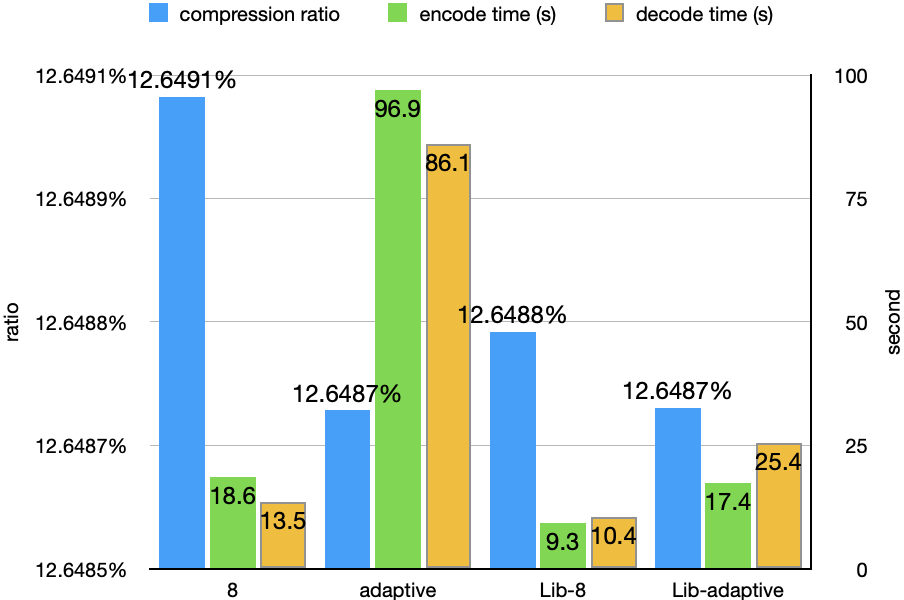
\includegraphics[height=6.15cm, keepaspectratio,]{assets/chart-compare-lib.png}}
\caption{The compression ratio and time compare with libcoders \cite{libcoders}.}
\label{fig-chart-compare-lib}
\end{figure}


\begin{figure*}[htbp]
\centerline{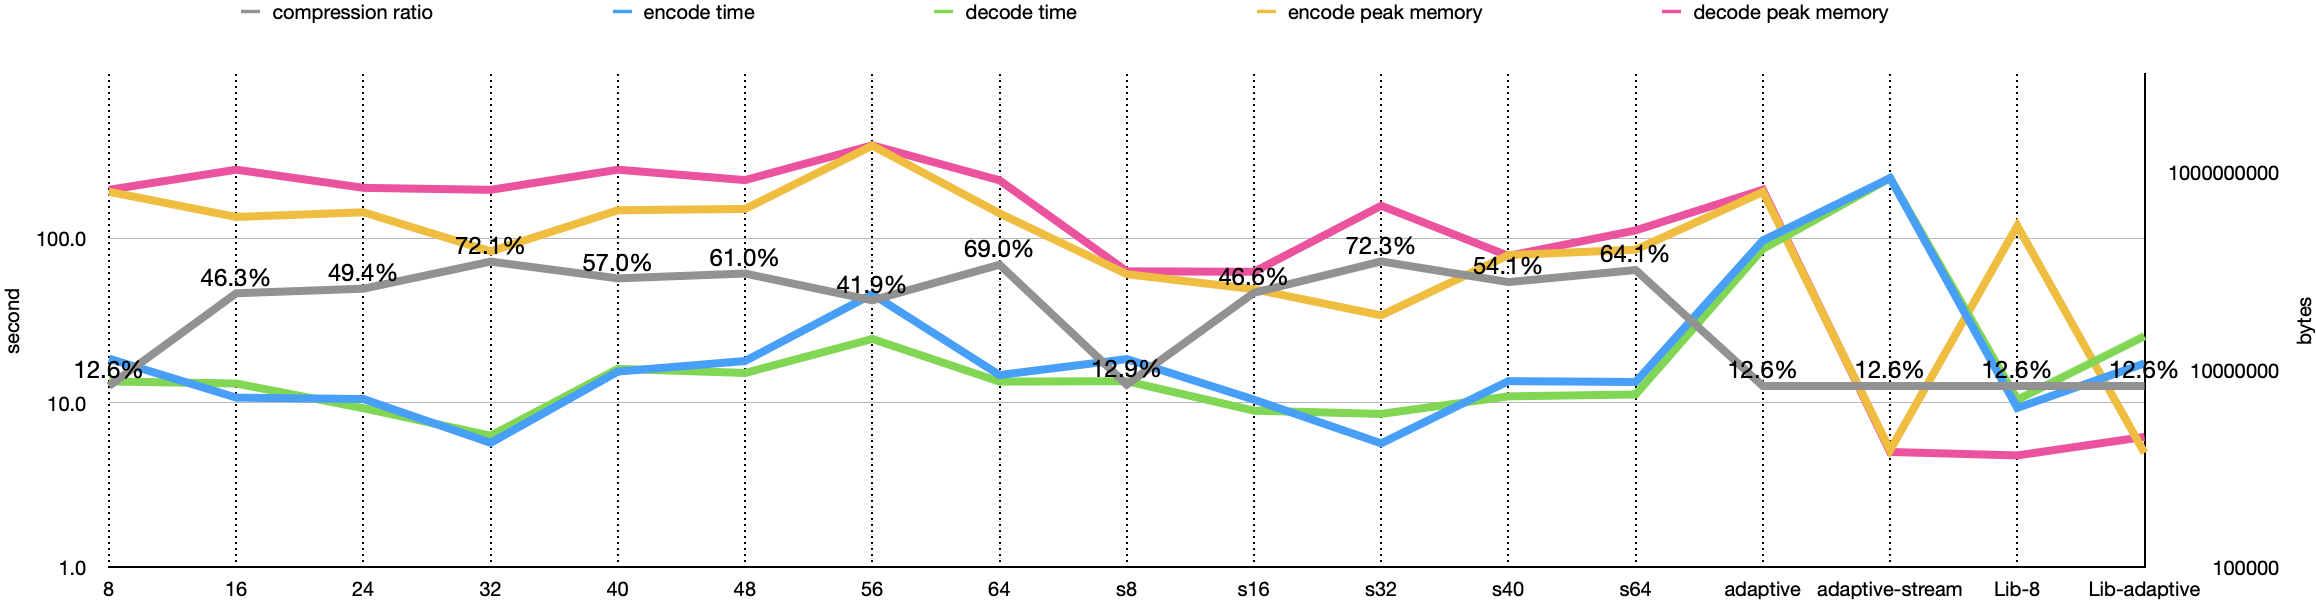
\includegraphics[width=20cm, keepaspectratio,]{assets/chart-time-memory.png}}
\caption{The time and memory usage of different algorithms and parameters.}
\label{fig-chart-time-memory}
\end{figure*}

We can see that the compression ratio of basic Huffman algorithm is slightly higher than libcoders, and the encode time and decode time of basic Huffman algorithm is a little higher than libcoders, and the peak memory usage of basic Huffman algorithm is higher than libcoders when decode.

We can see that the compression ratio of adaptive Huffman algorithm is same as libcoders, and the encode time and decode time of adaptive Huffman algorithm is much higher than libcoders, and the peak memory usage of adaptive Huffman algorithm is much higher than libcoders when non-stream output mode, and the peak memory usage of adaptive Huffman algorithm is same as libcoders when stream output mode.

\section{Conclusion}

In this homeowrk, I have implemented basic Huffman algorithm and adaptive Huffman algorithm, and compare with libcoders \cite{libcoders}. The result shows that the compression ratio of basic Huffman algorithm is slightly higher than libcoders, but program performance and memory usage have a lot of room for improvement.

\section{Appendix}

\subsection{Experiment Environment}

\begin{itemize}
\item CPU: Apple M1 Pro 8-Core (6 Performance / 2 Efficiency)
\item Memory: 16GB
\item Compiler: Apple clang version 14.0.3 \\ (clang-1403.0.22.14.1)
\item Measurement: /usr/bin/time -l -h -p
\end{itemize}

\subsection{Usage}

\begin{lstlisting}[escapeinside={(*}{*)}]
Usage: ./bin/release/huffman-coding.exe -t <type> [-e | -d] [options...] [-i <file>] [-o <file>]
    -t, --type <type>       Set coding algorithm
    -e, --encode            Encode
    -d, --decode            Decode
    -i, --input <file>      Set input file (default STDIN)
    -o, --output <file>     Set output file (default STDOUT)
    --ostream               Output stream
    -b, --bits <bits>       Tread input file as <bits> data source (default 8)
    -s, --split <size>      Split input file every <size> bytes of data (default (*$\infty$*) )
    -v, --verbose           Show debug / analysis /time info
    --pmf                   Show pmf freq
    --no-time               No show time info
    -h, --help              Show this help

Coding Algorithms
    analysis    Analysis entropy
    basic       Basic Huffman Coding Algorithm (bits: 8 <= 8k <= 64)
    adaptive    Adaptive Huffman Coding Algorithm
    extended    Extended Huffman Coding Algorithm (TODO)
\end{lstlisting}

\begin{thebibliography}{00}
\bibitem{efficient-way-of-storing-Huffman-tree} \url{https://stackoverflow.com/questions/759707/efficient-way-of-storing-Huffman-tree\#759766}
\bibitem{Introduction to Data Compression} Sayood, K. (2014), Introduction to Data Compression (4th Edition). Morgan Kaufmann
\bibitem{Wiki Adaptive_Huffman_coding} \url{https://en.wikipedia.org/wiki/Adaptive_Huffman_coding}
\bibitem{libcoders} \url{https://github.com/snovvcrash/libcoders/tree/master}
\end{thebibliography}

\end{document}
